\documentclass[margin=0pt]{standalone}

\usepackage{tikz}
\usetikzlibrary{backgrounds, matrix, patterns}

\begin{document}

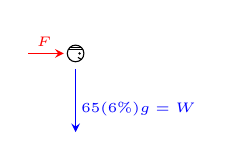
\begin{tikzpicture}
%Cabeza
\draw[fill=white] (0,0) circle (3pt);
\draw (-0.09,0.05) -- (0.09,0.05);
\draw (-0.07,0.075) -- (0.07,0.075);
\draw[fill=black] (0.05,0) circle (0.2pt);
\draw (0.07,-0.075) -- (0.03,-0.05);

%Vectores
\draw[red, -stealth] (-0.6,0) -- (-0.15,0);
\node[red] at (-0.4,0.15) {\tiny $F$};

\draw[blue, -stealth] (0,-0.2) -- (0,-1);
\node[blue] at (0.8,-0.7) {\tiny $65(6\%)g=W$};
\end{tikzpicture} 


\end{document}







